\chapter{Conceitos gerais e revisão da literatura}
Neste capítulo deve ser proporcionado o estado da arte / referencial teórico
sobre o tema a que se refere o estudo. Um bom pesquisador não deve repetir
trabalhos já concluídos ou que já estão em andamento. Por isso esta sessão é
onde o autor demonstra até onde vai a pesquisa atual no campo de estudos em
questão e estabelece as bases sobre as quais desenvolverá o estudo proposto. A
seguir são mostrados alguns exemplos de como deve-se inserir as figuras e
tabelas. A Figura \ref{fig:exemplo} mostra um exemplo de como inserir uma
figura no texto. A Tabela \ref{tb:exemplo} mostra o exemplo de como uma tabela
deve ser inserida.  Voce pode referenciar capítulos e seções adicionando labels
à elas. Por exemplo, descrevemos a introdução no Capítulo
\ref{chp:introduction}.

\begin{figure}[!htb]
    \centering
    \caption{Exemplo de como inserir Figura}
    
\includegraphics[width=0.45\textwidth]{images/figura.png}
    {\footnotesize Fonte: Inserir fonte conforme padrão ABNT.}
    \label{fig:exemplo}
\end{figure}

%Altere o numero junto ao 'width' para acertar o tamanho da figura. Coloque
%numeros maior que 0 e até 1


%Voce pode forcar a troca de pagina da seguinte forma:
\newpage

%Ao retirar figura de um site.
\begin{figure}[!htb]
    \centering
    \caption{Exemplo de como inserir Figura retirado de um site - Arduino Uno}
    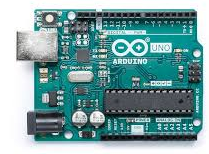
\includegraphics[width=0.35\textwidth]{images/uno.png}

    {\footnotesize Fonte: Página oficial do Arduino\protect\footnotemark}
    \label{fig:arduino_uno}
\end{figure}
\footnotetext{Disponível em: <https://www.arduino.cc/en/Main/ArduinoBoardUno>. Acesso em ago. 1999.}

\begin{table}[htb]
\caption{Modelo de como as tabelas devem ser inseridas no texto}
\label{tb:exemplo}
\centering
\begin{tabular}{|l|c|r|r|} %left, center, right. Você pode mudar isso
\hline
Índice  & Coluna 1 & Coluna 2 & Coluna 3 \\
\hline
Linha 1 &          &          &          \\
Linha 2 &          &          &          \\
Linha 3 &          &          &          \\
\hline
\end{tabular}
\end{table}
%Para manter a sanidade, recomenda-se deixar sempre os '&' alinhados em todas
%as linhas e colunas
